\chapter{Literature Review}
\label{chapter:literature}

{\color{red} TODO:
\begin{itemize}
    \item Overview of literature review section.
    \item Make nomenclature consistent with list of symbols.
\end{itemize}}


\section{Visual Question Answering Metrics}

In their seminal VQA paper, \citeauthor{malinowski2014multiworld} \cite{malinowski2014multiworld} note that traditional accuracy measures fail to capture partial correctness of answers; given a ground-truth answer `carton', the traditional accuracy metric would give zero weight to the answer `box', despite the semantic similarity between the ground-truth and predicted answers. In general, larger answer vocabularies typically lead to blurrier semantic boundaries between answer classes when compared to datasets with a smaller answer vocabulary like CIFAR \cite{krizhevsky2009learning}. Since datasets that frame the VQA problem as a classification task typically have a large answer vocabulary containing objects, numbers, colours and other concepts, it follows that an effective VQA metric should reward answers that are partially correct or share semantics with the ground-truth answer.

Metric design becomes even more important when considering full-sentence answers instead of single-word answers; evaluation of full-sentence answers requires metrics that are robust under semantic and syntactic variations between predicted and ground truth answers. A variety of natural language generation (NLG) metrics \cite{papineni2002bleu, lin2004rouge, banerjee2005meteor, vedantam2015cider} have been applied to image captioning tasks \cite{chen2015microsoft, vedantam2015cider}, and are consequently applicable to open-ended VQA tasks requiring full-sentence answers. Unfortunately, none of these metrics were designed explicitly for VQA tasks, and must be considered in addition to class-based metrics to gain useful insights into model performance. 

% Although I focus on VQA as a multi-class classification problem in this dissertation, I provide a brief overview of these metrics in \sectionautorefname{ \ref{subsection:open_ended_vqa_metrics}}, highlighting areas for further research into open-ended VQA metrics.

In the following subsections, I explore a variety of metrics for both class-based and free-form VQA tasks as outlined in \tableautorefname{ \ref{tab:vqa_metrics_suitability}}, focusing on how they reward partially correct answers.


\begin{table}[htbp]
    \centering
    \begin{tabularx}{\linewidth}{@{}lCCCl@{}}
        \toprule
        \multicolumn{1}{c}{\multirow{2}{*}{\textbf{Metric}}} & \multicolumn{3}{c}{\textbf{Suitability}}                                                           & \multicolumn{1}{c}{\multirow{2}{*}{\textbf{Common Uses}}} \\ \cmidrule(lr){2-4}
        \multicolumn{1}{c}{}                                 & \multicolumn{1}{c}{Multi-class} & \multicolumn{1}{c}{Multi-label} & \multicolumn{1}{c}{Open-ended} & \multicolumn{1}{c}{}                                      \\ \midrule
        Accuracy                                             & \checkmark                      & \checkmark                      &                                & Multiple                                                  \\
        WUPS                                                 & \checkmark                      & \checkmark                      &                                & Multiple                                                  \\
        Consensus Accuracy                                   & \checkmark                      & \checkmark                      &                                & VQA                                                       \\
        Consistency                                          & \checkmark                      & \checkmark                      &                                & VQA                                                       \\
        Validity                                             & \checkmark                      &                                 &                                & VQA                                                       \\
        Plausibility                                         & \checkmark                      &                                 &                                & VQA                                                       \\
        Grounding                                            & \checkmark                      & \checkmark                      & \checkmark                     & VQA                                                       \\
        Distribution                                         & \checkmark                      &                                 &                                & VQA                                                       \\
        BLEU \cite{papineni2002bleu}                                                &                                 &                                 & \checkmark                     & Machine translation                                       \\
        ROUGE \cite{lin2004rouge}                                                &                                 &                                 & \checkmark                     & Text summarisation                                        \\
        METEOR \cite{banerjee2005meteor}                                              &                                 &                                 & \checkmark                     & Machine translation                                       \\
        CIDEr \cite{vedantam2015cider}                                               &                                 &                                 & \checkmark                     & Image captioning                                          \\ \bottomrule
    \end{tabularx}
    \caption[Suitability of metrics for various VQA tasks]{A comparison of metrics and their suitability for various VQA tasks.}
    \label{tab:vqa_metrics_suitability}
\end{table}

\begin{table}[htbp]
    \begin{footnotesize}
      \begin{tabularx}{\linewidth}{@{}lLL@{}}
        \toprule
            \multicolumn{1}{c}{\textbf{Metric}} & \multicolumn{1}{c}{\textbf{Advantages}}                                                    & \multicolumn{1}{c}{\textbf{Disadvantages}}                                                                                                                              \\ \midrule
            Accuracy                            & - Simple and interpretable.                                                                & - Penalises slightly incorrect answers harshly.                                                                                                                         \\
                                                & - Suitable for problems with a small answer set cardinality.                               & - Requires an exact set of answers for multi-label tasks.                                                                                                               \\ \midrule
            WUPS                                & - Rewards incorrect but semantically similar answers.                                      & - Rewards answers that share a concept class \textit{e.g.} \textit{`colour'} with the true answer but have opposite meanings e.g. \textit{`white'} vs \textit{`black'}. \\ \midrule
            Consensus Accuracy                  & - Simple and interpretable.                                                                & - Multiple correct reference answers may be contradictory.                                                                                                              \\
                                                & - Aligns with human answers.                                                               & - Not all questions have 3 matching reference answers                                                                                                                   \\
                                                &                                                                                            & - Reference answers are expensive to collect.                                                                                                                           \\ \midrule
            Consistency                         & - Ensures models avoid contradictory answers to related questions.                         & - Requires a set of entailed questions for each question.                                                                                                               \\
                                                &                                                                                            &                                                                                                                     \\ \midrule
            Validity                            & - Measures a model's ability to respond to various question types.                         & - Requires a set of valid answers for each question type.                                                                                                               \\ \midrule
            Plausibility                        & - Ensures models avoid nonsensical answers.                                                & - Requires scene graphs for all dataset samples.                                                                                                                        \\
                                                &                                                                                            & - Can be imprecise for sparsely occurring objects.                                                                                                                      \\ \midrule
            Grounding                           & - Ensures models use image data to answer questions instead of exploiting language priors. & - Only applicable to attention-based models.                                                                                                                            \\
                                                &                                                                                            & - Requires knowledge about which image regions are relevant to each dataset sample.                                                                                     \\ \midrule
            Distribution                        & - Ensures models respond well to all question subject-type groups                          & - Cannot be compared across datasets with different distributions.                                                                                                                                                                       \\ \midrule
            BLEU                                & - \(n\)-grams capture positional relationships between words.                              & - Requires multiple ground truth answers for good performance.                                                                                                          \\
                                                & - Penalises answers that are too short or too long.                                        & - Performs better for entire corpora compared to individual sentences due to the corpus-level brevity penalty, an issue for VQA.                                        \\
                                                &                                                                                            & - A zero score for any \(n\)-gram component gives a zero BLEU score.                                                                                                    \\\bottomrule
    \end{tabularx}
    \end{footnotesize}
    \caption[Advantages and disadvantages of metrics for various VQA tasks]{A comparison of metrics and their advantages and disadvantages for various VQA tasks.}
    \label{tab:vqa_metrics_comparison}
\end{table}

\subsection{Semantic Similarity Measures}

\subsubsection{Wu-Palmer Similarity}

Originally coined the ``conceptual similarity measure'' \cite{wu1994verbs}, the now-labelled Wu-Palmer (WUP) similarity is used to measure the semantic similarity of two concepts based on their positions in a taxonomy tree such as WordNet \cite{miller1995wordnet}. Formally, given two concepts \(A\) and \(B\) in a taxonomy tree \(T\), we define the Wu-Palmer similarity of \(A\) and \(B\) as

\begin{equation}
    WUP(A, B) = \frac{2 N_C}{N_A + N_B + 2 N_C}
    \label{equation:wup}
\end{equation}

where \(N_A\) and \(N_B\) are the number of edges from \(A\) and \(B\) to their lowest common ancestor \(C\) respectively, and \(N_C\) is the depth of \(C\) in \(T\), as illustrated in \figureautorefname{ \ref{fig:wups_tree}}.

\begin{figure}[H]
    \centering
    \begin{forest}
      [ROOT [C, edge=dashed, edge label={node[midway,auto]{\(N_C\)}} [A, edge=dashed, edge label={node[midway,left]{\(N_A\)}}] [B, edge=dashed, edge label={node[midway,right]{\(N_B\)}}]]]
    \end{forest}
    \caption[A taxonomy tree describing the relationship between two concepts.]{Given two concepts \(A\) and \(B\), \(C\) denotes the ``least common superconcept'' of A and B. (Figure adapted from \cite{wu1994verbs})}
    \label{fig:wups_tree}
\end{figure}

Given this definition, it naturally follows that two equal concepts occupy the same position in the taxonomy tree and thus have a similarity of 1, whilst two concepts whose lowest common ancestor is the root of the tree have a similarity of 0.

Whilst WUP similarity can capture similarities between a target and predicted concept, \citeauthor{malinowski2014multiworld} extend WUP similarity to sets of concepts, proposing the WUP set score for evaluation of multi-label classification tasks:

\begin{equation}
    \textsc{WUPS}(A, B) = \frac{1}{N} \sum_{i=1}^N \min \{\prod_{a \in A_i} \max_{b \in B_i} \textsc{WUP}(a, b), \prod_{b \in B_i} \max_{a \in A_i} \textsc{WUP}(a, b)\}
    \label{equation:wups}
\end{equation}

To apply this metric to VQA tasks, we let \(A\) and \(B\) be a collection of sets of predicted and ground-truth answers respectively, each of size \(N\). Noting that \(WUP(A_i, B_i) \in [0, 1]\) for each \(A_i \in A\) and \(B_i \in B\), the following useful properties of the metric become evident:

\begin{enumerate}
    \item \(WUPS(A, B) \in [0, 1]\), with \(WUPS(A, B) = 1\) when \(A = B\).
    \item Naive models which overestimate the number of target answers will be penalised according to how dissimilar the additional provided answers are to their closest target answer.
    \item Models which underestimate the number of target answers \textit{i.e.} \(|A_i| < |B_i|\) will be penalised, with a harsher penalty if the concepts in the target set are dissimilar.
\end{enumerate}

The authors note that WUP yields large values for related but not interchangeable concepts, noting that \(WUP(\text{carton}, \text{box}) = 0.94\) where \(WUP(\text{stove}, \text{fire extinguisher}) = 0.82\). To encourage precise answers and avoid accepting related but inaccurate answers, the authors down-weight \(WUP(a, b)\) by a ratio \(r = 0.1\) whenever it is less than some threshold \(t = 0.9\).

While this down-weighting alleviates this issue for questions that query objects in an image, answers to questions about object attributes and colours are often poorly evaluated; \citeauthor{kafle2017visual} note that even after down-weighting \(WUP\) scores, \(WUPS(\text{white}, \text{black}) = 0.91\). Whilst the metric correctly rewards the answerer for correctly identifying that the answer to the question is a colour, a score of 0.91 seems too high, highlighting the non-linearity of the metric that makes it more difficult to interpret at a glance unlike other common metrics like accuracy.

By nature, the metric also operates on single WordNet concepts, which often coincide with single words. To evaluate full-sentence or even multi-word answers with WUPS, we must treat sentences as a set of distinct words, disregarding essential syntactic and contextual information. This makes WUPS a poor candidate for open-ended VQA evaluation when compared to other NLG metrics such as BLEU, ROUGE, METEOR and CIDEr, as briefly discussed in \subsectionautorefname{ \ref{subsection:open_ended_vqa_metrics}} and summarised in \tableautorefname{ \ref{tab:vqa_metrics_comparison}}.

%In addition to this issue, the down-weighting approach introduces two new parameters which increase the complexity and subjectivity of the metric. 


% \[
% \min \{\prod_{a \in A_i} \max_{b \in B_i} WUP(a, b), \prod_{b \in B_i} \max_{a \in A_i} WUP(a, b)\} =  \begin{cases}
%     1, &\text{if } A_i = B_i \\
%     \prod_{b \in B_i} \max_{a \in A_i} WUP(a, b) < 1, &\text{if } A_i \subset B_i \\
%     \prod_{a \in A_i} \max_{b \in B_i} WUP(a, b) < 1, &\text{if } A_i \supset B_i
% \end{cases}
% \]

\subsection{Consensus Measures}
\label{subsection:consensus_measures}

\subsubsection{VQA Consensus Accuracy}
Introduced by \citeauthor{antol2015vqa} in \citeyear{antol2015vqa}, the VQA consensus accuracy metric is the most common metric used to benchmark VQA models, due to the widespread adoption of the VQA dataset and its variants. To reward partially correct answers, VQA consensus accuracy compares a candidate answer to multiple reference answers, provided by humans via crowdsourcing platforms like Amazon Mechanical Turk (AMT) in the case of the VQA dataset. The VQA consensus accuracy metric is defined as

\begin{equation}
    \textsc{Accuracy} = \min \left( \frac{n}{3}, 1 \right)
    \label{equation:vqa_consensus_accuracy}
\end{equation}

where \(n\) is the number of answers in the set of reference answers that match a given candidate answer, \textit{i.e.} an answer is considered entirely correct if it matches 3 or more of the 10 reference answers for the corresponding question and image.

At a surface level, the metric is interpretable and can reward multiple correct and/or partially correct answers effectively, however, the latter can become a disadvantage depending on the quality of the reference answers. In their analysis of the VQAv1 dataset, \citeauthor{kafle2017visual} point out that 16.7\% of questions have less than 3 matching answers in their group of 10 reference answers, capping the performance of a perfect VQA model. A large contributor to this statistic is the presence of multi-word answers in the dataset; 89.32\% of answers in the VQAv1 dataset are single-word answers, leaving ample room for disagreement amongst reference answers.

Moreover, supporting multiple correct answers is unfavourable if the correct answers are contradictory. Again, \citeauthor{kafle2017visual} identify that 13\% of VQA v1 yes/no questions contain both `yes' and `no' 3 or more times in their group of 10 reference answers, making both options entirely correct.


% \begin{itemize}
%     \item ``Inter-human agreement is only 83.3\%. It is impossible for an algorithm to achieve 100\% accuracy.''\cite{kafle2017visual} % no consensus answer problem
%     \item even when counting only those answers in the VQAv2 training set that appear more than 8 times, there are still 3129 unique reference answers. After this selection,  \cite{teney2018tips}.
% \end{itemize}

\subsubsection{DAQUAR Consensus Measures}

Motivated by the relatively poor human baseline performance (Accuracy: 50.20\%, WUPS@0.9:  50.82\%) on the DAQUAR dataset, \citeauthor{malinowski2015ask} extended the dataset by collecting an average of 5 reference answers for each image-question pair and developing two consensus metrics based on their previous WUPS measure:

\begin{equation}
    \textsc{WUPS}_{\text{mean}}(A, B) =     \frac{1}{NK} \sum_{i=1}^N \sum_{i=1}^K \min \{\prod_{a \in A_i} \max_{b \in B_i} \textsc{WUP}(a, b), \prod_{b \in B_i} \max_{a \in A_i} \textsc{WUP}(a, b)\}
    \label{equation:wups_mean_consensus}
\end{equation}


\begin{equation}
    \textsc{WUPS}_{\text{min}}(A, B) =     \frac{1}{N} \sum_{i=1}^N \max_{k=1}^K \left( \min \{\prod_{a \in A_i} \max_{b \in B_i} \textsc{WUP}(a, b), \prod_{b \in B_i} \max_{a \in A_i} \textsc{WUP}(a, b)\} \right)
    \label{equation:wups_min_consensus}
\end{equation}

where \(N\), \(A\) and \(B\) are as defined in \equationautorefname{ \ref{equation:wups}}, and \(K\) is the number of reference answers for the \(i\)-th dataset sample.

The mean consensus metric rewards candidate answers that coincide with more frequent reference answers, whilst the minimum consensus metric rewards candidate answers according to their similarity to the closest reference answer.

\subsection{Metrics for Visual Reasoning}
\label{subsec:visual_reasoning_metrics}
As discussed earlier, the standard accuracy metric penalises partially correct answers as harshly as incorrect answers. When using accuracy alone, it is impossible to distinguish between a model that provides reasonable but incorrect answers and one that provides nonsensical answers. Moreover, the standard accuracy metric gives no insights into how a VQA model arrived at its answer to a given question and image.

To combat these issues, \citeauthor{hudson2019gqa} developed five new metrics in tandem with their GQA dataset \cite{hudson2019gqa} to evaluate the internal reasoning processes of VQA models: Consistency, Validity, Plausibility, Grounding and Distribution.

\subsubsection{Consistency}

The consistency metric is motivated by the following scenario:

Say we have two questions \(q_0\) and \(q_1\) that ask about properties of the same image, \textit{e.g.} \(q_0 = \)\textit{`What colour is the apple?'} and  \(q_1 = \) \textit{`Is the apple red?'}

Since both questions are asking about the same apple, a consistent model is one that does not contradict itself in answering the two questions \textit{e.g.} \(a_0 =\) \textit{`red'} and \(a_1 =\) \textit{`yes'} are consistent answers, where \(a_0 =\) \textit{`red'} and \(a_1 =\) \textit{`no'} are not.

To calculate consistency, each question-answer pair \(q, a\) in the GQA dataset is annotated with a set of entailed questions \(E_q\). For the example above, \(q_1\) is an entailed question of \(q_0\), since knowing the answer to \(q_0\) infers the answer to \(q_1\). Given a the set of questions \(Q\) that a model answered correctly and a set entailed questions for each \(q \in Q\) denoted \(\mathcal{E} = \{E_q \mid q \in Q\}\), the consistency metric is calculated according to \algorithmcfname{ \ref{algorithm:consistency}}.

\begin{algorithm}[htbp]
    \caption[Consistency metric algorithm]{Consistency metric algorithm}
    \label{algorithm:consistency}
    \Function{\(Q, \mathcal{E}\)}{
        \(s_c \leftarrow 0\)\\
        \ForEach{\(\{q_i \in Q \mid E_{q_i} \neq \emptyset\}\)}{
            \(s_{q_i} \leftarrow 0\)\\
            \ForEach{
                \(q_e \in E_{q_i}\)
            }{
                \lIf{
                    \(q_e \in Q\)
                }{
                    \(s_{q_i} \leftarrow s_{q_i} + 1\)
                }
            }
            \(s_c \leftarrow s_c + \frac{s_{q_i}}{|E_{q_i}|}\)
        }
        \Return \(\frac{s_c}{|\{q_i \in Q \mid E_{q_i} \neq \emptyset\}|}\)
    }
\end{algorithm}

% On 4000 random questions of the GQA dataset, \citeauthor{hudson2019gqa} report a human consistency of 98.4, and accuracy of 89.3, indicating that humans are mostly consistent but not always accurate in their responses.

Unfortunately, the consistency metric does not account for inaccurately answered questions. There is certainly an argument to be made that including incorrect answers in the consistency calculation would skew the consistency metric in favour of more accurate models. Moreover, including these incorrect answers could give large consistency scores for poorer models that exploit statistical priors in the dataset's answer distribution.
Nonetheless, knowing consistency amongst incorrectly answered questions gives information about the model's overall reasoning skills and tendency to exploit statistical biases in certain question types. Hence, for error analysis purposes, it would be more suitable to compute consistency over incorrectly answered questions instead of computing consistency over all questions.

% Multi-question learning?

\subsubsection{Validity}

The validity metric is the most lenient of the GQA metrics, and simply captures whether a candidate answer corresponds with the type of answer the question demands. For example, valid answers for questions starting with \textit{What colour} are colours like \textit{red} or \textit{blue}, where answers like \textit{yes} or \textit{three} would be invalid.

To calculate validity, the GQA evaluation script \cite{hudson2019evaluation_script} contains a set of valid answers \(V_q\) for every question in the dataset. For each question \(q \in Q\) and its corresponding candidate answer \(\hat{a}_q\), the validity metric is simply:

\begin{equation}
    \textsc{Validity} = \frac{1}{|Q|}\sum_{q \in Q} \begin{cases}
        1, &\text{if } \hat{a}_q \in V_q\\
        0, &\text{otherwise }\\
    \end{cases}
    \label{equation:validity}
\end{equation}

\subsubsection{Plausibility}

Where the validity metric aims to measure whether answers to questions are non-degenerate, plausibility measures whether the candidate answer is rational by checking for co-occurrence of the answer and the question's subject in the scene graphs for the rest of the dataset.

In practice, plausibility is computed in the same way as validity, using a pre-computed set of plausible answers \(P_q\)  for each question in place of the set of valid answers \(V_q\) used in \equationautorefname{ \ref{equation:validity}}.

The method used to compute \(P_q\) for each question depends on the question's type; for the GQA dataset, the scene graph contains attributes, objects and relations, meaning that plausibility needs to be computed differently depending on whether the question's answer is an object, relation or attribute. Moreover, plausibility also needs to be computed for other types of questions whose answers are not in the scene graph, such as binary and counting type questions.

For the sake of brevity, I will focus on two different question types to give an intuition about how sets of plausible answers are determined.

For questions that ask about an attribute of an object \(o\), an attribute is considered plausible if it co-occurs with \(o\) at least once in the scene graphs for other images in the dataset. For example, \textit{red} would be a plausible answer to the question \textit{What colour is the apple?} if the dataset contains at least one image of a red apple, where \textit{blue} would be implausible.

For questions that ask about a target object \(t\) given a subject \(s\) and relation \(r\) \textit{e.g. What is the man holding?}, \(t\) is considered plausible if there exists a relation \(s, r, t\) in the scene graph for any image in the dataset. 

\subsubsection{Grounding}

The grounding measure is unlike other metrics in that it does not compare the quality of answers given by a VQA model. Instead, it focuses on model interpretability, ensuring models use relevant visual information to formulate answers. For example, consider a model that can answer the majority of questions about the colour of an apple correctly based purely on the fact that the most common answer to such questions is red; such a model does not utilise any visual information in its reasoning process. Conversely, a model that answers the same proportion of questions correctly by identifying the location and colour of apples in an image is a visually \textit{grounded} model, and exhibits the type of behaviour that we strive for as a research community.

At its core, the grounding metric takes as input a set of sets of bounding boxes \(\hat{\mathcal{B}} = \{\hat{B}_{(q_i, r_i)} \mid ((q_i, r_i), a_i) \in S\}\) for each question-image pair \((q_i, r_i)\) in a VQA dataset \(S = \{((q_i, r_i), a_i)\}_{i=1}^n\). Each bounding box in \(\hat{B}_{(q_i, r_i)}\) corresponds to a region in the image \(r_i\) that the the model attended to when answering the associated question \(q_i\). Moreover, each bounding box \(\hat{b} \in \hat{B}_{(q_i, r_i)}\) has an associated attention value \(\alpha_{\hat{b}}\), indicating the importance assigned to that image region by the model during the question-answering process. These predicted bounding boxes and attention values are compared to a set of sets of reference bounding boxes \(\mathcal{B} = \{B_{(q_i, r_i)} \mid ((q_i, r_i), a_i) \in S\}\), where each box in \(B_{(q_i, r_i)}\) indicates the visual regions in \(r_i\) that are essential for answering question \(q_i\).

The grounding metric for any \((q_i, r_i)\) pair in a dataset is defined as the total precision-based overlap between each set of predicted and reference regions \(\hat{B}_{(q_i, r_i)}\) and \(B_{(q_i, r_i)}\) respectively. For an entire dataset \(S\), per-sample grounding scores are averaged to give the final grounding metric, as outlined in \algorithmautorefname{ \ref{algorithm:grounding}}.

\begin{algorithm}[htbp]
    \caption[Grounding metric algorithm]{Grounding metric algorithm}
    \label{algorithm:grounding}
    \Function{\(S, \hat{\mathcal{B}}, \mathcal{B}\)}{
        \(s_g \leftarrow 0\)\\
        \ForEach{\(((q_i, r_i), a_i) \in S\)}{
            \(B \leftarrow B_{(q_i, r_i)} \in \mathcal{B}\)\\
            \(\hat{B} \leftarrow \hat{B}_{(q_i, r_i)} \in \hat{\mathcal{B}}\)\\
            \ForEach{\(b \in B\)}{
                \ForEach{\(\hat{b} \in \hat{B}\)}{
                    \(\alpha_{\hat{b}} \leftarrow \text{Attention coefficient for } \hat{b}\)\\
                    \(s_g \leftarrow s_g + \alpha_{\hat{b}} \times \frac{\text{IntersectionArea}(\hat{b}, b)}{\text{Area}(\hat{b})}\)
                }   
            }
        }
        \(s_g \leftarrow \frac{s_g}{n}\)\\
        \Return \(s_g\)
    }
% # compare attention map to gold regions
% scores = []
% for region in regions:
%     for cell, attention in cells:
%         scores.append(attention * intersectionRate(cell, region))
% return sum(scores)
\end{algorithm}

Unfortunately, any VQA model that does not use attention-based mechanisms to attend to regions or objects in an image cannot be evaluated using the grounding metric. This limitation is becoming more important, as more recent models have adopted graph-based representations of visual inputs instead of spatial or object-based image features. For this reason, I do not report grounding metric results for my model in \chapterautorefname{ \ref{chap:results}}.

\subsubsection{Distribution}

Given the importance of dataset balancing and the influence of language priors on model performance as discussed in \sectionautorefname{ \ref{section:vqa_datasets}}, the distribution metric compares the distributions of reference and candidate answer sets. This provides a way of measuring whether a VQA model exploits statistical priors and focuses on more common answers or whether it can predict less-frequent answers based on its knowledge of the question and image.

The similarity score of the candidate and reference distributions for each question type is computed using the Pearson Chi-squared statistic \cite{pearson1900x}, and the distribution metric is a weighted average of these scores, with the weights being the number of questions of that type. I refer the reader to \cite{hudson2019gqa} for detailed analysis of question type distributions in the GQA dataset.

\subsection{Metrics for Open-ended VQA}
\label{subsection:open_ended_vqa_metrics}

Given the challenge of multi-class and multi-label VQA tasks, there has been little research into open-ended VQA task, even though some datasets contain full-sentence answers for each question. In addition, research into open-ended VQA has been stunted by the lack of a widely accepted metric for the task; metrics such as BLEU, ROUGE, METEOR and CIDEr were originally developed for other tasks as shown in \tableautorefname{ \ref{tab:vqa_metrics_suitability}}, and thus have various disadvantages when used in VQA contexts.

Since I focus on VQA as a multi-class classification problem in this dissertation, I keep this section brief, delving into the characteristics of BLEU to exemplify the types of issues that open-ended VQA evaluation poses. I choose to elaborate on BLEU instead of metrics with more robust characteristics like ROUGE, METEOR and CIDEr since BLEU was used for evaluation of early open-ended VQA datasets such as Visual Madlibs \cite{yu2015visual}. Moreover, since BLEU suffers from multiple weaknesses \cite{banerjee2005meteor} in the context of machine translation, it serves as a good example to illustrate common points of consideration for more advanced metrics. For the keen reader, I outline some of the key shortcomings of the BLEU metric that metrics like ROUGE, METEOR and CIDEr address at the end of this subsection.

\subsubsection{BLEU}

Originally developed for automatic evaluation of machine translation systems, the Bi-Lingual Evaluation Understudy (BLEU) metric was created in an effort to reduce dependence on manual evaluation methods and thus promote more rapid prototyping of ideas. The three keys to its success in the machine translation field are its efficiency, language independence and correlation with human evaluation results.

In the context of machine translation, the core component of the BLEU metric compares groups of \(n\) adjacent words (\(n\)-grams) in a candidate translation to \(n\)-grams in a group of reference translations using a modified precision measure. This comparison is best described with an example:

\begin{table}[htbp]
    \centering
    \begin{tabular}{r|l}
        Candidate & \textbf{the} \textbf{the} the the the the the \\
        Reference 1 & \textbf{the} cat is on \textbf{the} mat \\
        Reference 2 & there is a cat on the mat \\
    \end{tabular}
    \caption[An illustration of BLEU's modified \(n\)-gram precision measure \cite{papineni2002bleu}]{An example given by \cite{papineni2002bleu} of a poor candidate translation that performs well \((7/7)\) on the standard unigram precision measure, but poorly \((2/7)\) on the modified unigram precision measure used by BLEU.}
    \label{tab:bleu_ngraph_precision}
\end{table}

As illustrated in \tableautorefname{ \ref{tab:bleu_ngraph_precision}}, the standard \(n\)-gram precision measure simply counts how many \(n\)-grams in the candidate translation appear in any of the reference translations, allowing poor translations that repeat common \(n\)-grams to perform well. To combat this, the BLEU metric uses a modified \(n\)-gram precision measure, where it calculates a clipped number of \(n\)-gram matches between the candidate and reference translations: in the example in \tableautorefname{ \ref{tab:bleu_ngraph_precision}}, the unclipped candidate count of the unigram \textit{the} is 7, but the clipped count is 2, since the maximum number of occurrences of the unigram \textit{the} in any reference translation is 2.

\cite{papineni2002bleu} extend their modified \(n\)-gram precision measure to multiple sentences, however I omit this section for the sake of clarity since open-ended VQA answers are almost always phrased as single sentences.

Whilst these modified \(n\)-gram precisions are useful for gaining an idea of whether a candidate translation is good or bad, the BLEU metric accounts for the fact that different\(n\)-gram precisions capture different aspects of a translation. For example, unigram precision is useful for measuring whether a candidate translation uses the same words as a reference translation, but cannot account for the \textit{fluency} of a translation like bigram or trigram precisions can. To address this, the BLEU metric combines multiple modified \(n\)-gram precision scores according to \equationautorefname{ \ref{equation:bleu_metric}}.

\begin{equation}
    \textsc{BLEU} = P_B \cdot \exp \left(\frac{1}{N} \sum_{n=1}^N \log p_n\right)
    \label{equation:bleu_metric}
\end{equation}

In \equationautorefname{ \ref{equation:bleu_metric}}, we see that the BLEU metric is defined as some brevity penalty \(P_B\) multiplied by the geometric mean of individual \(n\)-gram precisions \(p_n\). This brevity penalty is essential for ensuring candidate translations are not too short; a candidate translation can achieve a modified precision score of 1 if it contains a single \(n\)-gram and that \(n\)-gram is in one of the reference answers. The brevity penalty achieves this by comparing the length of the candidate translation \(c\) to the length of the reference translation closest in length to \(c\), denoted \(r\), taking a value \(< 1\) whenever \(c < r\). Moreover, the penalty decays exponentially towards zero as \(c \rightarrow 0\), as seen in \equationautorefname{ \ref{equation:bleu_brevity_penalty}}.

\begin{equation}
    P_B = \begin{cases}
    1, &\text{if } c > r\\
    e^{\frac{1-r}{c}}, &\text{if } c \leq r\\
    \end{cases}
    \label{equation:bleu_brevity_penalty}
\end{equation}

Naturally, the BLEU metric can be used for any natural language evaluation task where we need to compare a candidate sentence to a reference sentence. This includes open-ended VQA evaluation, where we compare sentence-based candidate answers to one or more reference answers.

Analysing the design decisions of the BLEU metric, we see that it handles a variety of issues that apply to open-ended VQA evaluation. Firstly, it encourages responses of appropriate length; the brevity penalty ensures that candidate responses are not too short, and the modified \(n\)-gram precision measure inherently penalises responses that include superfluous \(n\)-grams not found in reference responses. This ensures that candidate responses not only get the question correct, but provide an answer in the context of a sentence. Secondly, by including \(n\)-gram precision measures for multiple values of \(n\), it ensures candidate answers are correct and fluent in their vocabulary usage.

Unfortunately, there are numerous disadvantages to using the BLEU metric for open-ended VQA evaluation, some of which have been addressed by one or more of ROUGE, METEOR and CIDEr.
Firstly, VQA datasets rarely contain multiple open-ended answers. For example, the GQA dataset \cite{hudson2019gqa} comes with a single open-ended answer per question. This means that a candidate answer that is correct but differs in phrasing to the reference answer may achieve a low BLEU score. This occurs because BLEU was originally designed for large corpora with multiple reference translations sourced from different people to promote answer variety. Even the more recent CIDEr metric is consensus based, requiring multiple image captions to evaluate the quality of a candidate description. To effectively utilise metrics like BLEU and CIDEr for open-ended VQA tasks, it is essential to have multiple candidate answers for each question in the dataset.
Secondly, the BLEU metric does not account for synonyms or morphological variations of words. If the ground truth answer refers to a \textit{carton} but the predicted answer uses the word \textit{box}, or \textit{cartons}, we observe a decrease in \(n\)-gram precision despite the semantic or morphological similarities between words used by the candidate and reference answers. This issue is addressed in the METEOR and CIDEr metrics, making them more robust to candidate answer phrasing variations.
Moreover, we see that open-ended VQA answers often have a large overlap with their corresponding question. For example, given the question \textit{What colour is the apple?} and a reference answer \textit{The apple is red.}, a candidate answer \textit{The apple is.} would achieve a modified unigram, bigram and trigram precision of 1 despite drawing all of its words from the question and not providing a concrete answer. This emphasises the importance of using regular multi-class VQA metrics like accuracy, validity and plausibility in tandem with NLG metrics, as a high BLEU, ROUGE, METEOR or CIDEr score may not necessarily correspond to a correctly answered question. This makes it difficult to compare the performance of VQA models since there is no one-size-fits-all metric for open-ended VQA evaluation.


% For some \(n \geq 1\), the BLEU metric defines the modified \(n\)-gram precision as \(p_n = \frac{\sum{c \in C} \sum g_n \in c }{\sum{c' \in C} \sum g_n' \in c}\), where \(C\) is a set of candidate answers

% \textbf{Motivations:}

% \begin{itemize}
%     \item Machine translation
%     \item Human evaluation can take months
%     \item Bi-Lingual Evaluation Understudy (BLEU) is:
%     \begin{itemize}
%         \item ``Quick''
%         \item ``Inexpensive''
%         \item ``Language independent''
%         \item Accurate (``Correlates highly with human evaluation'')
%     \end{itemize}
%     \item 
%     \item Derived from word-error-rate metric used in speech recognition, modified to allow for subtle word reorderings and substitutions.
% \end{itemize}


% \textbf{General Caveats:}

% \begin{itemize}
%     \item Relies on multiple ground truth sentences with different flavours/styles (translations for NMT, answers for VQA or image captioning). BLEU does better on a large corpus than for individual sentences.
%     \item Performs better for entire corpora compared to individual sentences due to the corpus-level brevity penalty.
%     \item Brevity penalty is required to avoid short answers like \textit{of the}, where there is only one \(2\)-gram which is likely to occur in ground truth answers but contains no useful contextual information.
% \end{itemize}


% \textbf{Application to VQA:}

% Brevity penalty in the context of VQA:

% {\color{red} TODO: Check image captioning paper and see if this is the adopted approach. Also check DAQUAR and COCO-QA papers.} Assume a candidate answer may contain multiple sentences and a ground truth answer may contain multiple sentences. In the most common case, the number of sentences in both the candidate and ground truth answers is 1. For cases with multiple sentences we can treat multiple sentences as a single sentence when computing \(n\)-grams, as in \cite{papineni2002bleu}. For a candidate answer of length \(c\) and a reference answer length of \(r\) (for each candidate sentence, the reference length is the corresponding ground-truth sentence with the closest length. \(r\) is the sum of these reference lengths across all sentences in the corpus, though the corpus is small for VQA applications.) The brevity penalty \(P_B\) is thus:

% \begin{equation}
%     P_B = \begin{cases}
%     1, &\text{if } c > r\\
%     e^{\frac{1-r}{c}}, &\text{if } c \leq r\\
%     \end{cases}
%     \label{equation:bleu_brevity_penalty}
% \end{equation}

% \begin{itemize}
%     \item Relies on multiple ground truth sentences with different flavours/styles (translations for NMT, answers for VQA or image captioning). BLEU does better on a large corpus than for individual sentences.
%     \item Performs better for entire corpora compared to individual sentences due to the corpus-level brevity penalty.
%     \item Brevity penalty is required to avoid short answers like \textit{of the}, where there is only one \(2\)-gram which is likely to occur in ground truth answers but contains no useful contextual information.
% \end{itemize}


% \subsubsection{ROUGE}

% \textbf{Motivations:}

% \begin{itemize}
%     \item Recall based rather than precision-based like BLEU. For text summarisation we generally prefer a candidate summary that covers a consensus of ground-truth answers.
%     \item Different variations:
%     \begin{itemize}
%         \item \textsc{Rouge-N}: ``\(n\)-gram recall between a candidate summary and set of reference summaries''
%     \end{itemize}
% \end{itemize}

% \textbf{General Caveats:}

% \begin{itemize}
%     \item 
% \end{itemize}

% \textbf{Application to VQA:}

% Assume the following notation:

% \(S\) is a set of ground-truth summaries (answers in the context of VQA) for a given dataset sample.

% \(c\) is a candidate summary, \textit{e.g.} one produced by a model.

% \(g_n\) is an \(n\) gram contained within a single summary \(s \in S\). In practice, each summary may contain multiple sentences, in which case \(n\)-grams are not computed across sentence boundaries, but for open-ended VQA answers, we can assume the answer is short and can be expressed as a single sentence.

% \begin{equation*}
%     \textsc{ROUGE -N} = {\arg \max}_{s\in S} \frac{
%         \sum_{g_n \in s} \min \left(\text{Count}_s(g_n), \text{Count}_c(g_n) \right)
%     }{
%         \sum_{g_n \in s} \text{Count}_s(g_n)
%     }
% \end{equation*}

% For VQA with a single one-sentence reference answer and one-sentence candidate answer, \textsc{Rouge-N} is simply \(n\)-gram recall.

% \subsubsection{METEOR}

% \textbf{Motivations:}

% \begin{itemize}
%     \item 
% \end{itemize}

% \textbf{General Caveats:}

% \begin{itemize}
%     \item 
% \end{itemize}

% \textbf{Application to VQA:}
% \begin{itemize}
%     \item 
% \end{itemize}

% \subsubsection{CIDEr}

% \textbf{Motivations:}

% \begin{itemize}
%     \item 
% \end{itemize}

% \textbf{General Caveats:}

% \begin{itemize}
%     \item 
% \end{itemize}

% \textbf{Application to VQA:}
% \begin{itemize}
%     \item 
% \end{itemize}


\section{Visual Question Answering Datasets}
\label{section:vqa_datasets}

In this section, I address the first major hurdle for the VQA task as introduced in \chapterautorefname{  \ref{chapter:introduction}}: \textit{How do we design a dataset that effectively captures subtle relationships between questions and images as presented in real-world situations where VQA would prove useful?} Effectively answering this question requires answering multiple related sub-questions:

\begin{enumerate}
    \item What kind of images represent the situations in which we would use VQA models, and how do we gather these types of images?
    \item What kind of questions would humans ask about these images and how can they be collected?
    \item How do we ensure that the answer distribution for the dataset reflects the types of answers we see to questions in the real world whilst not over- or under-representing certain answer types?
\end{enumerate}

I address the first two of these questions in \subsectionautorefname{ \ref{subsection:question_and_image_collection}}, outlining the wide variety of approaches to image and question collection and/or generation employed by a variety of datasets. In \subsectionautorefname{ \ref{subsec:lanauge_priors_in_vqa_datasets}}, I emphasise the importance of the final question, describing strategies used by dataset creators to ensure question and answer distributions accurately represent our observations of the real world and explain how statistical imbalances in question and answer distributions can lead to an overly-optimistic evaluations of VQA model performance.

\subsection{Collecting Questions and Images for VQA Datasets}
\label{subsection:question_and_image_collection}

Naturally, the first design decision to make when designing a VQA dataset is to determine the type of questions and images to use and how to gather them. As illustrated in \figureautorefname{ \ref{fig:dataset_samples}} in the introduction, different datasets take different approaches to image and question collection, depending on the type of visual reasoning skills they wish to test. For example, the VQAv1 \cite{antol2015vqa} and v2 \cite{goyal2017making} datasets contains photographs of many real-world  scenarios in which VQA may prove useful for helping the visually-impaired, including busy urban areas and rooms within people's homes. Other datasets adopt a different approach, using images of scenes assembled from 2D clip art objects \cite{zitnick2013bringing, antol2015vqa}, shapes \cite{andreas2016neural}, or assorted 3D solids with various colours \cite{johnson2017clevr}. These datasets provide a standard benchmark for assessing the reasoning capabilities of different VQA models, and are thus not viable training signals for real-world VQA applications. Similarly, many datasets collect questions for each image via crowdsourcing platforms like Amazon Mechanical Turk (AMT) in order to simulate the types of questions that humans wish to ask in the real world. Others like CLEVR \cite{johnson2017clevr} and GQA \cite{hudson2019gqa} generate questions using a combination of templates and scene graph information, intentionally avoiding the inherent ambiguity of questions created by humans and instead focusing on how well VQA models are able to interpret and understand complex questions syntax.

I summarise the most common VQA datasets along with their image sources, question creation methods and other features in \tableautorefname{ \ref{tab:dataset_comparison}}, before delving into the question and image collection methods and motivations behind the most influential VQA datasets.


% More formally, we wish to develop a dataset \(\mathcal{X}\) such that \(x \sim \mathcal{D}\ \forall x \in \mathcal{X}\) for some fixed, underlying distribution \(\mathcal{D}\) \cite{mohri2018foundations}. For a dataset to be \textit{useful}, we require that \(\mathcal{D}\) captures the distribution of real-world VQA problems that we wish to solve.
%\(S \in ( \times \mathcal{Y})^n\) 

% The methods used to generate VQA datasets are as useful in understanding the relationship between images and questions as VQA models themselves; as an example, it is much easier to generate questions instead of images, the images for many VQA datasets have been drawn from existing image datasets such as COCO \cite{lin2014microsoft}, and questions have been generated using a variety of methods including crowd-sourcing, question templates, functional programs and scene graphs. By analysing the question generation process, it is possible to gain insights into how graphical and textual data is related in a question-answering context, and use this knowledge to analyse the effectiveness of the ways in which image and question data is processed for use by various VQA models. An overview of the most popular VQA datasets and their generation methods is provided in Table \ref{tab:dataset_comparison}, followed by a detailed deconstruction of the methods used and challenges addressed by their respective creators and how they relate to the interplay of images and text in visual reasoning tasks.

\begin{landscape}
  \begin{footnotesize}
        \begin{longtable}{
            P{0.15\linewidth}cccP{0.08\linewidth}P{0.07\linewidth}P{0.1125\linewidth}P{0.125\linewidth}P{0.1\linewidth}
        }
          \toprule
          \textbf{Dataset}
          & \textbf{Year}
          & \textbf{Images}
          & \multirow{2}{0.1\linewidth}{\centering\textbf{Question-\\Image Pairs}}
          & \textbf{Image Source}
          & \textbf{Question Creation}
          & \textbf{Answer Type}
          & \textbf{Additional Data}
          & \textbf{Evaluation Metrics}\\
          \midrule
          \endhead

          \bottomrule\\
          \caption[A comparison of VQA datasets and their variations.]{A comparison of relevant features of the most popular VQA datasets. Dataset variations are listed in regular font below their bolded counterparts. For clarity, I make the distinction between single-concept and open-ended VQA tasks:  what many datasets call an \textit{open-ended} VQA task is a task requiring a short 1-3 word (\textit{single-concept}) answer. Most often, these types of tasks are approached as a classification problem across the entire answer vocabulary of the dataset. I reserve the \textit{open-ended} answer type for VQA tasks that require full-sentence answers.}
          \label{tab:dataset_comparison}
          \endlastfoot

          \textbf{DAQUAR} \cite{malinowski2014multiworld}
          & 2014
          & 1,449  % 1449 images
          & 12,468  % 12,468 questions
          & NYU-Depth V2 \cite{silberman2012indoor}
          & Both
          & Multi-label (894)
          & Human segmentation, image depth values, and object labels from NYU Depth V2.
          & Accuracy, WUPS \\
        \midrule
          \textbf{Visual Madlibs} \cite{yu2015visual}
          & 2015
          & 10,738  % 10,738 images  % Filtered hard task?
          & 360,001  % 360,001 descriptions
          & COCO
          & Human
          & Fill-in-the-blank, Multi-choice (4)
          & COCO annotations
          & Accuracy, BLEU \\
          \midrule
          \textbf{COCO-QA}\cite{ren2015exploring}
          & 2015
          & 123,287
          & 117,684
          & COCO
          & Automatic
          & Single-concept
          & COCO annotations
          & Accuracy, BLEU \\
          \midrule
          \textbf{VQAv1} \cite{antol2015vqa}
          & 2015
          & 204K  % 204,721 images
          & 614K  % 614,163 questions % 6,141,630 ground truth answers % 1,842,489 plausible answers
          & COCO
          & Human
          & Single-concept, Multi-choice (18)
          & COCO image captions
          & Accuracy, Consensus Accuracy\\
          Abstract Scenes
          & 2015
          & 50K  % 50,000 abstract scenes
          & 150K  % 150,000 questions % 1,500,000 ground truth answers % 450,000 plausible answers % 250,000 captions
          & 2D clip art
          & Human
          & Single-concept, Multi-choice (18)
          & Image captions
          & Accuracy, Consensus Accuracy\\
          Changing Priors (CP) \cite{agrawal2018dont}
          & 2018
          & \(\approx\)204K  % Exact unkown as calculation was based on sum of train and test which are not necessarily mutually exclusive on images.
          & \(\approx\)370K  % Exact unkown, ~ 3.8M answers
          & COCO
          & Human
          & Single-concept
          & See VQAv1
          & Consensus Accuracy \\
          Compositional VQA (C-VQA) \cite{agrawal2017cvqa}
          & 2017
          & 204K  % Some images repeated in train and test
          & 369K  % 369,861 questions, 3,698,610 answers
          & COCO
          & Human
          & Single-concept
          & See VQAv1
          & Consensus Accuracy \\
          \midrule
          \textbf{VQAv2} \cite{goyal2017making}
          & 2017
          & 204K  % 204,721 images
          & 1.1M  % 1,105,904 questions % 11,059,040 ground truth answers
          & COCO
          & Human
          & Single-concept
          & COCO image captions, complementary image pairs
          & Accuracy, Consensus Accuracy \\
          Balanced Binary Abstract Scenes \cite{zhang2016yin}
          & 2016
          & 31K % 31,325 abstract scenes
          & 33K % 33,383 questions % 333,830 ground truth answers
          & 2D clip art
          & Human
          & Multi-choice (2)
          & Image captions
          & Accuracy \\
          Changing Priors (CP) \cite{agrawal2018dont}
          & 2018
          & \(\approx\)204K  % Exact unkown as calculation was based on sum of train and test which are not necessarily mutually exclusive on images.
          & \(\approx\)658K  % Exact unkown, ~ 6.6M Answers
          & COCO
          & Human
          & Single-concept
          & See VQAv2
          & Consensus Accuracy  \\
          \midrule
          \textbf{Visual Genome} \cite{krishna2017visual}
          & 2016
          & 108K  % 108,077 images
          & 1.7M  % 1,773,258 questions and answers
          & COCO, YFCC100M \cite{thomee2016yfcc100m}
          & Human
          & Single-concept
          & COCO annotations, region descriptions, scene graphs
          & Accuracy \\
          \midrule
          \textbf{Visual7W} \cite{zhu2016visual7w}
          & 2016
          & 47K % 47,300
          & 327K % 327,939
          & COCO
          & Human
          & Single-concept, Multi-choice (4)
          & Groundings for each object in each question-answer pair.
          & Accuracy \\
          \midrule
          \textbf{TDIUC} \cite{kafle2017analysis}
          & 2017
          & 167K % 167,437 images
          & 1.6M % 1,654,167 questions
          & COCO, Visual Genome
          & Both
          & Single-concept
          & See Visual Genome.
          & Per-question-type accuracy, regular \& normalised arithmetic \& harmonic mean accuracy\\
          \midrule
          \textbf{CLEVR} \cite{johnson2017clevr}
          & 2017
          & 100K  % 100,000 images
          & 999K  % 999,968 questions
          & 3D renderings
          & Automatic
          & Single-concept
          & Functional programs, scene graphs
          & Accuracy \\
          CoGenT-A \& B
          & 2017
          & 100K
          & 999K
          & 3D renderings 
          & Automatic
          & Single-concept
          & Functional programs, scene graphs
          & Accuracy \\
          Humans
          & 2017
          & 32K  % 32,164
          & 32K  % 32,164
          & CLEVR
          & Human
          & Single-concept
          & See CLEVR.
          & Accuracy \\
          \midrule
          \textbf{GQA} \cite{hudson2019gqa}
          & 2019
          & 113K  % 113,018 images
          & 22.6M  % 22,669,678 questions
          & COCO, Visual Genome
          & Both
          & Single-concept, open-ended
          & Scene graphs, functional programs, full-sentence answers, valid and plausible answer sets for each question, entailed questions, faster R-CNN \cite{ren2016faster} features, ResNet-101 \cite{he2016deep} features, ground-truth bounding boxes.
          & Accuracy, Consistency, Validity, Plausibility, Distribution, Grounding \\
      \end{longtable}
  \end{footnotesize}
\end{landscape}

\subsubsection{DAQUAR}

As the first of many VQA datasets, \textit{the DAtaset for QUestion Answering on Real-world images} (DAQUAR) was born from a desire to combine the advances of the computer vision (CV) and natural language processing (NLP) communities and tackle more complex problems. DAQUAR draws its images from the NYU-Depth V2 dataset, utilising its depth information to automatically segment and classify objects in the image. Interestingly, DAQUAR employs both question templates for automatic question generation as well as human-provided questions and answers, separating them into ``SynthQA'' and ``HumanQA'' benchmarks respectively.

Whilst ahead of its time, DAQUAR has two primary issues that have hindered its widespread adoption:
\begin{enumerate}
    \item \textbf{Size}: As shown in \tableautorefname{ \ref{tab:dataset_comparison}}, DAQUAR contains only 1,449 images and 12,468 questions. This makes it infeasible for modern deep-learning based methods and also limits the ability for VQA models trained on DAQUAR to generalise to new question-image pairs.
    \item \textbf{Question Variety}: Whilst there is plenty of variety in the ``HumanQA'' benchmark, images in the ``SynthQA'' benchmark are associated with one of four question types, each with their own template as shown in \tableautorefname{ \ref{table:daquar_templates}}.
\end{enumerate}


\begin{table}[htbp]
    \centering
    \begin{tabular}{cl}
        \toprule
        \textbf{Question Type} & \textbf{Template} \\
        \midrule
        Counting & How many \{object\} are in \{image\}?\\
        Counting with colours & How many \{colour\} \{object\} are in \{image\}?\\
        Room type & Which type of the room is depicted in \{image\}?\\
        Superlative comparison & What is the largest \{object\} in \{image\}?\\
        \bottomrule
    \end{tabular}
    \caption[DAQUAR Question templates from, adapted from \cite{malinowski2014multiworld}]{DAQUAR question templates from the ``SynthQA'' benchmark that target the contents of a single image, adapted from \cite{malinowski2014multiworld}.}
    \label{table:daquar_templates}
\end{table}

% \textbf{VQAv1} \cite{antol2015vqa} Real images were drawn from COCO \cite{lin2014microsoft}, and . Questions and answers were collected using an Amazon Mechanical Turk (AMT) interface.

% \textbf{VG} \cite{krishna2017visual} Images from the intersection of COCO \cite{lin2014microsoft} and YFCC100M \cite{thomee2016yfcc100m}. Questions, answers and scene graphs were collected using an AMT interface.

% \textbf{V7W} \cite{zhu2016visual7w} Images are a subset of the Visual Genome dataset. Questions, answers and object-level groundings were collected using an AMT interface.

% \textbf{VQAv2} \cite{goyal2017making, zhang2016yin} Built on top of VQA 1.0, new (image, question, answer) tuples were created from existing tuples by asking AMT workers to choose an image from 24 nearest neighbours of the existing tuple's image such that the answer to the new image is not the answer to the existing image for the same question.

% \textbf{TDIUC} \cite{kafle2017analysis} Questions were collected from COCO-QA and VG, generated from COCO and VG segmentation and object/attribute annotations respectively, or created by human volunteers. Images from COCO and VG were used if associated with a question.

% \textbf{GQA} \cite{hudson2019gqa} Scene graphs were created using various preprocessing techniques from VG scene graphs. Questions were produced compositionally from combinations of templates derived from VQA 2.0 and manually-created templates, using scene graph traversals to fill in subjects, objects, relations and attributes, whilst simultaneously filling in the functional program templates associated with the question types. An additional balancing helped mitigate statistical priors that are often exploited by models, whilst maintaining real-world priors.

\subsubsection{VQAv1}

Given the rise in popularity of VQA tasks inspired by DAQUAR, \citeauthor{antol2015vqa} recognised a need for a new, sufficiently large dataset that contained free-form, open-ended questions that still allowed results to be quantified; this need was realised by two datasets: an open-ended dataset derived from COCO \cite{lin2014microsoft}, as well as a smaller synthetic dataset containing abstract scenes assembled from 2D clip-art objects \cite{zitnick2013bringing}. These datasets are referred to as VQAv1 and Abstract Scenes (listed underneath VQAv1) in \tableautorefname{ \ref{tab:dataset_comparison}} respectively. The key contributions of these datasets are two-fold:

\begin{enumerate}
    \item The real-world image dataset provided the first feasible dataset for benchmarking VQA models, thanks to its large size compared to existing VQA datasets like DAQUAR and COCO-QA. Whilst smaller, the synthetic abstract scenes dataset allowed researchers to investigate the underlying theory behind visual reasoning without focusing on the difficult task of extracting features from images.
    \item Both datasets employed a new consensus accuracy metric that rewards models for feasible answers based answers given by 10 human volunteers. Whilst not a perfect metric due to the small number of collected human answers, the authors correctly emphasise that metrics such as BLEU and ROUGE from other NLP tasks are not suited to the dataset, since the answers to questions are only ever single concepts, spanning 1-3 words. As a result, this consensus accuracy has been widely adopted as a standard metric for the evaluation of VQA systems. I refer the reader to \subsectionautorefname{ \ref{subsection:consensus_measures}} for details on the consensus accuracy metric.
\end{enumerate}

Despite the large success and valuable contributions of the VQAv1 dataset, it suffers from large statistical biases in its answer set distribution. As an example, \cite{goyal2017making} points out that a VQA model that answers \textit{yes} to any question beginning with \textit{Do you see a ...} in the VQAv1 dataset achieves a consensus accuracy of 87\% on those questions. This is largely due to the question generation process and general human disposition; humans are much more likely to ask the question \textit{Do you see a dog?} if there is actually a dog in the image compared to if there is not. These skewed answer distributions encourage models to rely on question language priors and answer distribution priors to formulate answers without properly incorporating image data into their reasoning processes. I delve further into the impact of language priors in \subsectionautorefname{ \ref{subsec:lanauge_priors_in_vqa_datasets}}, focusing on dataset balancing methods developed by other dataset creators to help capture the observations we see in the real world more accurately.

\subsubsection{CLEVR}
Motivated by the prevalance of skewed answer and question distributions in existing datasets, \citeauthor{johnson2017clevr} built the CLEVR dataset to help diagnose common issues and limitations with existing VQA models. They took an entirely different approach to question and image collection, automating both processes to give complete control over question, image and answer distributions.

The key to automating question and image generation is the scene graph, a representation of an image's objects, their attributes and their relationships to other objects. Each object is represented as a node in the scene graph and is annotated with zero or more attributes, and inter-object relationships are represented as  graph edges. Scene graphs were made popular in the VQA field by the Visual Genome dataset, but had been previously used for image retrieval tasks \cite{johnson2015image}. I refer the reader to \subsectionautorefname{ \ref{subsection:scene_graph_embedding_motivation}} for a formal description of a scene graph and its components.

The creation of each question-image pair in the CLEVR dataset begins with a randomly generated scene graph containing objects \textit{e.g. cube, sphere, cylinder}, attributes \textit{e.g. colour, material and size} and inter-object relationships \textit{e.g. left, right, in front, behind, same attribute}. Scene graph objects and their associated attributes are placed on a 2D plane, positioned according to the relationships encoded by the scene graph, and then rendered using Blender's Python API \cite{blender}. 
Questions are drawn from a collection of around 360 templates, each of which is associated with a functional program. Choosing elements from the scene graph to populate the template and functional program results in a fully-formed question and functional program describing the reasoning processes required to answer the question for that scene graph. For example, the question template \textit{How many \{colour\} things are there?} is associated with a functional program \texttt{count(filter\_colour(\{colour\}, scene))}. To obtain an answer to a question-image pair, the associated functional program is evaluated on the scene graph to yield an object, attribute or relation.

The main issue with the CLEVR dataset as a whole is its limited vocabulary. This leads to reasonably simple images that provide easily distinguishable visual signals based on object and attribute type, as well as an extremely limited answer vocabulary when compared to other VQA datasets. This is clearly seen in the extremely low error rates of VQA models on the dataset; not long after the creation of CLEVR, FiLM \cite{perez2017film} obtained an overall accuracy of 97.7. This was swiftly beaten by \citeauthor{hudson2018compositional}'s Compositional Attention Network \cite{hudson2018compositional}, which achieved an overall accuracy of 98.9 in \citeyear{hudson2018compositional}.

\subsubsection{GQA}
Inspired by the complex compositional structure of questions in the CLEVR dataset and motivated by the lack of question annotations and suboptimal question and answer distributions in existing datasets, \citeauthor{hudson2019gqa} developed the GQA dataset. GQA is the largest VQA dataset to date, containing over 22 million questions in entirety, and over 1.7 million questions after applying balancing techniques to reduce biases in its question type and answer distributions. Moreover, it is accompanied by a myriad of additional annotations, ranging from scene graphs, functional programs and full-sentence answers to Faster R-CNN object features and ResNet-101 spatial features.

At a glance, the GQA dataset construction process comprises four key stages:

\begin{enumerate}
    \item Scene graph preprocessing
    \item Question creation
    \item Entailment relation discovery
    \item Dataset balancing
\end{enumerate}

Due to the complexity of the GQA dataset construction process, I provide a brief overview of these four key steps below. I refer the avid reader to the original GQA publication \cite{hudson2019gqa} for unabridged details on the construction of the GQA dataset.

\textbf{Scene graph preprocessing:} Similarly to CLEVR, scene graphs are the starting point for the creation of the GQA dataset. Instead of randomly creating scene graphs and generating images from these graphs, the GQA dataset draws 113K images and scene graphs from the Visual Genome (VG) dataset. Like CLEVR scene graphs, these graphs contain objects, attributes and relations. In addition to spatial relations like \textit{left, right, etc.} as seen in the CLEVR dataset, the VG scene graphs contain verbal \textit{e.g. using, holding, wearing} and comparative \textit{e.g. larger than, shorter than, higher than} relationships. Hierarchical classification techniques and word embedding distances are used to consolidate the natural language used across the VG scene graphs, giving a final vocabulary of 1740 objects, 620 attributes and 330 relations across all dataset splits. After vocabulary creation, the authors remove incorrect and/or unnatural \textit{e.g. (man, in, shirt)} relations between objects using both manual and automatic methods. Finally, additional spatial relationships are added to the scene graph based on object bounding box information, and global properties about the scene are stored alongside each scene graph.

\textbf{Question creation:} As seen in previous works, the GQA dataset uses a set of 524 question templates as the heart of its question generation process, 274 of which were created by creating templates from existing VQAv1 questions. In addition to substituting objects, attributes and relations into question templates, entire sub-templates can be substituted to create complex, compositional questions of varying lengths. For example, the question \textit{"Are there napkins under the utensil to the left of the rice?"} may have been generated from the template \textit{Are there \{object\} \{preposition\} the \{object\}?}, where the first object placeholder was replaced with \textit{napkins}, but the second object placeholder was replaced with a sub-template \textit{the \{object\} \{relation\} the \{object\}?}. Moreover, some question templates support random omission or substitution of phrases or expressions. To avoid answer distribution imbalance for logical questions requiring object/attribute existence, decoy objects or attributes are sometimes substituted into question templates. For example, in the VQAv1 dataset, we saw that questions of the form \textit{Do you see a \{object\}...} are correctly answered with \textit{yes} 87\% of the time. Substituting the object reference with a decoy object that is not a part of the scene graph, 50\% of the time provides control over the answer distribution for those types of questions, as well as over object and attribute occurrence and co-occurrence probabilities.

\textbf{Entailment relation discovery:} Prior to question generation, each question template is associated with a functional program that describes the reasoning operations required to answer the question. My substituting objects, attributes, relations and sub-programs during the question generation phase, a functional program for each question-image pair is created. By categorising each of these functional programs, the authors determine which types of questions are answerable given the answer to another question on the same image. For example, if we know the answer to the question \textit{What colour is the apple?}, then we can guarantee we know the answer to the question \textit{Is the apple green?}. These entailment relations enable the GQA consistency metric as described in \subsectionautorefname{ \ref{subsec:visual_reasoning_metrics}}, as well as fine-grained analysis of the types of questions that VQA models find trivial or difficult.

\textbf{Dataset balancing:} \citeauthor{hudson2019gqa} take a different approach to answer distribution balancing, first smoothing the answer distribution based on global answer types \textit{e.g. colour, material} and then by local answer types which include information about the question subject \textit{e.g. colour-apple} for the question \textit{What colour is the apple?}. Global smoothing penalises VQA models that choose the most common answer for certain question structures, and local smoothing makes it more difficult to guess answers based on the subject of a question. This smoothing is performed by reweighting each global or local conditional distribution so that more frequent answers become less frequent and vice versa, whilst maintaining the frequency-ranked order of answers for each bin. Most importantly, this process is tunable, allowing fine control over the balance between uniformity of answer distributions and closeness to real-world distributions. As a result, at the time of writing, I consider \citeauthor{hudson2019gqa}'s implementation of answer distribution balancing as the most appropriate answer to my 3rd question for effective VQA dataset creation, as posed at the start \sectionautorefname{ \ref{section:vqa_datasets}}.

\subsection{Language Priors and Answer Distributions in VQA Datasets}
\label{subsec:lanauge_priors_in_vqa_datasets}

As briefly mentioned in the previous \subsectionautorefname, answer distribution and question type distribution have a significant impact on model evaluation. Skewed question and answer distributions are clearly seen in early VQA datasets, but as the first widely accepted VQA dataset, the VQAv1 dataset brought these issues to the forefront of the VQA field. Many prominent authors \cite{agrawal2016analyzing, zhang2016yin, kafle2017visual, goyal2017making, johnson2017clevr, agrawal2018dont, hudson2019gqa} have noted that VQA models will exploit statistical priors present in textual information and often neglect visual information if given the opportunity. To encourage the creation of VQA models that learn useful visual reasoning skills, VQA dataset authors aim to create datasets that contain minimal evaluation-hindering biases, whilst staying true to observations that we see in real-world situations.

As an example of this trade-off, consider the question \textit{What colour is the apple?}. A dataset where the answer to this question is \textit{red} 80\% of the time and \textit{green} 15\% of the time and \textit{yellow} 5\% of the time could be considered biased, since a VQA model could simply identify the type of question and blindly answer \textit{red} to achieve an accuracy of 80\% on these questions. However, balancing the dataset's answer distribution is not as simple as making the answer distribution uniform, since the real world has its own priors. In the real world, the distribution of red, green and yellow apples is dependent on apple variety, ripeness and growing conditions, and is likely not uniform.

In the remainder of this \subsectionautorefname, I will explore a variety of techniques used by different dataset creators, highlighting their novelties and downfalls.

\textbf{VQAv2}\\
Since its creation, many researchers have created variations and derivatives of the VQAv1 dataset, creating different types of questions \cite{agrawal2017cvqa}, alternative train and test splits with differing distributions \cite{agrawal2018dont} and smoothing out its skewed question and answer distributions \cite{zhang2016yin, goyal2017making}. The VQAv1 dataset creators highlight that VQA models can perform surprisingly well without any access to visual information; even a simple ``per-question type prior'' model achieves 71.03\% and 35.77\% on binary and numeric questions respectively, and an LSTM with only question word embeddings performs similarly at 78.20\% and 35.68\% \cite{antol2015vqa}. Two primary studies aim to solve these issues: the first \cite{zhang2016yin} focuses on the imbalance in the answer distribution of binary questions in the VQAv1 abstract scenes dataset, and the second \cite{goyal2017making} focuses on all question types in both the primary VQAv1 and VQAv1 abstract scenes datasets. The results of these two studies form the dataset now known as VQAv2, a popular benchmark for VQA systems on natural questions.

The first study is motivated by the large imbalance in the answer distribution of binary questions, noting that \textit{yes} is the answer to 68\% of all binary questions in the abstract scenes dataset. They propose a solution that allows the answer distribution of binary questions in the existing abstract scenes dataset to be balanced: for each question-image pair, they task humans with the creating a new scene using existing clip-art objects \cite{zitnick2013bringing} that is similar to the existing image, but had a complementary answer to the same question, as shown in \figureautorefname{  \ref{fig:zhang2016yin_balancing_procedure}} below.

\begin{figure}[H]
    \centering
    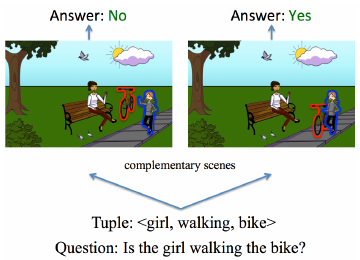
\includegraphics[width=0.5\textwidth]{zhang2016yin_balancing_procedure.png}
    \caption[A Technique for balancing answers to binary questions \cite{zhang2016yin}]{\citeauthor{zhang2016yin} \cite{zhang2016yin} demonstrate their answer distribution balancing technique. Given the scene on the left and the question \textit{Is the girl walking the bike}, workers were tasked with creating a scene that differs from the scene on the left but has the opposite answer to the question, as illustrated by the scene and answer on the right.}
    \label{fig:zhang2016yin_balancing_procedure}
\end{figure}

Though novel, this approach does not extend well to real-world image datasets, due to an inability to generate complementary images that are indistinguishable from photographs. Moreover, the approach is only applicable to binary questions, which comprise almost 41\% of the VQAv1 abstract scenes dataset \cite{antol2015vqa}. Despite this method's success in reducing the proportion of unbalanced question-image pairs by almost 72\%, around 20.48\% of question-image pairs in the balanced dataset were left unbalanced because they did not have a complementary image, either because a complementary scene could not be created due to limitations of the clip-art library (5.93\%) \textit{e.g.} a question such as \textit{`Is it raining?'} cannot be negated effectively, since the clip-art object bank does not contain a rain graphic, or due to disagreement between the answers collected by workers for a given scene (14.55\%)

For the rest of the questions in the VQAv2 dataset, \citeauthor{goyal2017making} use a similar approach, but instead of asking AMT workers to create a new image, they provide them with 24 nearest-neighbour images to choose from such that the answer to the new image is not the answer to the existing image for the same question. Answers to these new question-image pairs were collected in a similar fashion to the VQAv1 dataset. As a result, the number of question-image pairs in the VQAv2 dataset is almost double that of the VQAv1 dataset, and the frequency-weighted average entropy of answer distributions increased by 56\% due to the balancing process.

\textbf{GQA}\\
\citeauthor{hudson2019gqa} approach the task of dataset balancing from a different angle, aiming to mitigate biases in the answer distributions of the GQA dataset whilst maintaining some degree of representation of real-world priors. For brevity, I refer the reader to \subsectionautorefname{ \ref{subsection:question_and_image_collection}} for details on the balancing process used in the GQA dataset, as it is built-in to the dataset creation process.

% \subsubsection*{VQA: Visual Question Answering (\cite{antol2015vqa})}

% Given the underwhelming nature of existing visual question answering studies due to small datasets or restricted question or image contexts, the authors of this paper aim to create a diverse dataset that focuses on real-world questions about images. They created two datasets, one containing real-world images pulled from the MSCOCO dataset, and one containing abstract scenes to facilitate pioneering research into VQA tasks. The questions for both datasets were created by humans via an online interface, with a focus on question diversity and image relevance. In addition, ten answers for the questions were collected through a similar interface, and an accuracy metric was devised based on these human responses that accounts for variance in the quality of correct answers. Though this is necessary given the nature of the question generation process, the authors to not highlight why this accuracy metric was chosen over other alternatives; an important discussion given the subjective nature of answer quality. In addition, the question generation process resulted in answer distributions that are skewed towards a particular answer for many question types, encouraging models to rely on language priors to formulate answers without properly incorporating image data into their reasoning processes. However, to the authors' credit, these answer distributions are detailed meticulously in the appendices, but unfortunately these statistics do not find their way into the analysis of models found in many other papers, making it difficult to compare the extent to which different models take advantage of prior probabilities when answering questions.

% %%%%%

% \subsubsection*{Yin and Yang: Balancing and Answering Binary Visual Questions (\cite{zhang2016yin})}

% In this paper, the authors highlight the role of language priors in VQA dataset, providing concrete examples from the VQA 1.0 dataset (\cite{antol2015vqa}) where a simple model can form correct predictions solely based on question words; they show that these priors are present in multiple question types in the VQA 1.0 dataset, pointing out that questions starting with \textit{`What sport is'} can be correctly answered with the word \textit{`tennis'} 41\% of the time, and \textit{`yes'} is over twice as likely to be the answer to binary questions. The authors leverage the flexibility of abstract scenes in an attempt to eliminate language priors by modifying a copy of each image in the VQA abstract scenes dataset such the answer to the original question on the new image is negated. Though novel, this approach does not extend well to real-world image datasets, due to an inability to generate complementary images that are indistinguishable from photographs. Even with the benefits of abstract scenes, the balancing approach is unable to perfectly balance the binary portion of the dataset; for example, a question such as \textit{`Is it raining?'} cannot be negated effectively, since the clip-art object bank does not contain a rain graphic. Moreover, the approach is only applicable to binary questions, which comprise around 41\% of the VQA 1.0 dataset (\cite{antol2015vqa}). To demonstrate the effectiveness of this balancing technique, the authors compare the accuracy of four models when trained on the balanced and unbalanced binary question subset and tested on the unbalanced set of binary questions. They find that the language-only baseline suffers an 18\% decrease when trained on the balanced subset, and more complex models perform between 7-10\% worse. Whilst the paper presents a novel approach to VQA dataset balancing, its inability to completely balance binary questions in real and synthetic datasets alike makes it ineffective as a method for standardising VQA datasets.


% \subsubsection*{GQA: A New Dataset for Real-World Visual Reasoning and Compositional Question Answering (\cite{hudson2019gqa}), CVPR 2019}

% Given the prevalence of statistical biases present in other VQA datasets, \citeauthor{hudson2019gqa} provide a VQA dataset with compositional questions grounded on real-world images, balancing answer distributions during dataset creation. In addition, image scene graphs and functional programs are used as tools to create the dataset, as well as provide additional supervision options to potential models, and form a basis for new evaluation metics: distribution, grounding, validity, plausibility and consistency. The effectiveness of these metrics in evaluating VQA models is demonstrated by a set of baseline tests on probabilistic prior, vision-only (CNN), language-only (LSTM), naive language and vision (CNN+LSTM) and state-of-the-art attention base models (BottomUp and MAC). The balancing procedure used aims to find a balance between uniformly distributing answers for certain question types and maintaining relevant real-world priors by setting upper and lower bounds on the occurrence ratio of different answers for a given question type. Whilst this approach enables a tunable degree of distribution-balancing, the authors do not discuss how they determined the best parameters to use in this process, stating only that ``the entropy of the answer distribution increased by 72\%'' after balancing. One major improvement that \citeauthor{hudson2019gqa} make over the VQA datasets is that they leverage structured data in their new metrics, shifting focus from debates about what makes an `accurate' answer to more human-centered measures like how plausible, valid and consistent a model's answers are. Whilst these metrics are certainly useful, they are not usable in other datasets due to lack of information. This has made the comparison of SOTA models more complex, highlighting a need for frequent summaries of model performance on various relevant datasets. This need is further substantiated by the absence of questions requiring external or common-sense knowledge, such as \textit{`Why is it raining?'} or \textit{`What sound does the animal make?'}, as found in the original VQA datasets.


\section{Visual Question Answering Methods}
\label{section:vqa_methods}

Given the widespread adoption of scene graph annotations in VQA datasets \cite{krishna2017visual, zhu2016visual7w, johnson2017clevr, hudson2019gqa} it makes sense to leverage scene graph information for training VQA models. In previous years, many researchers have avoided using scene graphs as supervisory data, as they serve as an almost perfect visual signal. Additionally, scene graphs could not always be relied on as a supervisory data source; the scene graphs in the Visual Genome dataset were meticulously annotated by over 33,000 AMT workers \cite{krishna2017visual}, and the scene graphs in GQA required a large amount of additional pruning and modification to fit them to a standardised vocabulary of objects, relations and attributes. However, more recently, researchers have been using these datasets to develop scene graph generation methods \cite{xu2017scene, li2017scene, yang2018graph, tang2019learning}. As these scene graph generation methods become more accurate in their relationship existence and annotation methods, generated graphs as an image embedding will be more feasible, as they can be created quickly for any input image.

\subsubsection*{Image Representations}
\addcontentsline{toc}{subsubsection}{Image Representations}

\begin{itemize}
    \item CNN features
    \item Image object features and annotations
    \item Scene Graphs
\end{itemize}

\subsubsection*{Question Representations}
\addcontentsline{toc}{subsubsection}{Question Representations}

\begin{itemize}
    \item Traditional word embeddings e.g. word2vec, GloVe
    \item Recurrent neural network embeddings, e.g. LSTM, GRU and their bidirectional counterparts. 
    \item Dependency-based word embeddings \cite{levy2014dependency}
    \item Functional Programs
\end{itemize}

\subsubsection*{Combined Question and Image Representations}
\addcontentsline{toc}{subsubsection}{Combined Question and Image Representations}

\begin{itemize}
    \item Question-Image co-attention \cite{lu2016hierarchical}
    \item Bilinear models e.g. BLOCK Fusion \cite{ben2019block}
\end{itemize}




% \subsubsection*{Attention Mechanisms}
% \addcontentsline{toc}{subsubsection}{Attention Mechanisms}

% Attention mechanisms have gained traction in the research community recently, with the rise of non-recurrent models like the Transformer \cite{vaswani2017attention}, and pre-trained models like BERT \cite{devlin2018bert}. Many have realised their potential for multi-modal reasoning tasks, using a variety of attention-based mechanisms to aid reasoning processes.

% \vspace{\baselineskip}

% \citeauthor{hudson2018compositional} leverage the power of self-attention in their Memory-Attention-Composition cell, heavily inspired by recurrent architectures like LSTMs and GRUs. Aiming to shift the focus of VQA models from 
% Bottom-Up and Top-Down:

% MAC: Good, interpretable, but uses BiLSTM for embedding and raw spatial features. What about scene graphs and dependency-based embeddings? (BLOCK-MAC)

% DMCN: 

% DFAF:

% DCAF:

% Hierarchical Question-Image Co-Attention for Visual Question Answering

% - BLOCK:
%   - More efficient than simple bilinear models
%   - Fewer trainable parameters than other fusion techniques, yet outperforms six novel fusion methods.
%   - Not interpretable
  
% - MAC:
%   - Interpretable
%   - Does not use scene graphs or functional programs for supervision, however show a drastic improvement

% \subsubsection*{Multi-Modal Fusion}
% \addcontentsline{toc}{subsubsection}{Multi-Modal Fusion}

% BLOCK Superdiagonal Fusion: Performs decently in terms of VQA metrics, and performs much better than raw bilinear models, however is not interpretable.

% BAN: TODO

\subsection{Graph Methods}

Originally proposed for inductive and transductive node-classification tasks, the graph attention network (GAT) \cite{velivckovic2017graph} has gained the attention of computer vision researchers in the last three years, particularly for image-to-scene-graph \cite{yang2018graph} and text-to-scene-graph \cite{han2020victr} generation, and, more recently, visual question answering \cite{li2019relation, huang2020aligned}.
Prior works have demonstrated the effectiveness of attention-based graph convolutions for processing scene graph information in a variety of different contexts, with ReGAT \cite{li2019relation} achieving state-of-the-art results on the VQAv2 and VQA-CPv2 datasets in \citeyear{li2019relation}, and DC-GCN \cite{huang2020aligned} achieving comparable or greater performance than ReGAT on various VQAv2 subtasks in \citeyear{huang2020aligned}. However, both of these models do not evaluate the effectiveness of GATs for scene graph processing using gold-standard scene graph information. This makes it difficult to determine how much of the reported performance gain over non-scene-graph-based models can be accredited to the GAT architecture, and how much is due to the inclusion of generated scene graph information. In the following subsections, I outline how GCN and GAT architectures can be leveraged for VQA tasks, before giving a brief overview and analysis of the DC-GCN and ReGAT VQA architectures.

\subsubsection{Semi-Supervised Classification with Graph Convolutional Networks} \cite{kipf2016semi}
\label{kipf2016semi}
Originally proposed for graph-based semi-supervised classification tasks, the Graph Convolutional Network (GCN) extends the core concepts of Convolutional Neural Networks (CNNs) to sparse graphs; instead of performing convolutions on regions of pixels, GCNs convolve features from connected nodes in graphs.
{\color{red} TODO expand, including important features}

\noindent

\subsubsection{Graph Attention Networks} \cite{velivckovic2017graph}
\label{velivckovic2017graph}
{\color{red} TODO expand, including important features}

\subsubsection{Aligned Dual Channel Graph Convolutional Networks for VQA} \cite{huang2020aligned}
\label{huang2020aligned}

Current graph-based VQA methods focus only on capturing relationships between objects in images, and process textual information using traditional RNN-based approaches, indicating a need to close the semantic gap between question and image domains. \citeauthor{huang2020aligned} propose graphical representations of question data allow for multi-modal reasoning when reconciled with image objects. The authors of this paper have three main aims:

\begin{enumerate}
    \item To reconcile the objects and their relationships in images with words and their relationships in questions as a way of reasoning on multimodal data.
    \item To develop a method for generating meaningful graphical representations of question data for use in VQA tasks.
    \item To prove that graph-based methods perform on-par or better than existing SOTA VQA approaches.
\end{enumerate}

The methodology behind the model can be summarised as follows:

\begin{itemize}
    \item I-GCN
    \begin{itemize}
        \item Between 10 and 100 object proposals per image, each \(\in \R^{2048}\)
        \item Graphs edges are determined by bounding box intersection-over-union and a linear embedding of object vectors at the edge's endpoints.
    \end{itemize}
    \item Q-GCN
    \begin{itemize}
        \item Questions words represented with 300-dim GloVe embeddings \cite{pennington2014glove}, then encoded using an LSTM.
        \item Graph edge existence is determined using a Stanford dependency parser, and nodes store question word embeddings.
    \end{itemize}
    \item Attention alignment
    \begin{itemize}
        \item Self-attention on question words
        \item Attention on visual features using question attention results as a query.
        \item Linear multimodal fusion between attention outputs \(\tilde{H}_v\) and \(\tilde{H}_q\), with BCE loss computed over the candidate answer vocabulary:
        \[H_r = W_v^\top \tilde{H}_v + W_q^\top \tilde{H}_q\]
        \[softmax(W_e H_r + b_e)\]    
    \end{itemize}
\end{itemize}
Whilst one of the first methods to leverage graph strcutures for question embeddings, the scene graph generation method captures only naive spatial relations, compared to a model like ReGAT which models both explicit and implicit spatial and semantic relationships \cite{li2019relation}. Moreover, dependency-parsed graphs lack spatial and semantic information; they capture structural relationships between words that do not directly translate to spatial/semantic relationships in the joint question-image domain. In addition, the attention alignment module operates on two different data modes, each with their own semantic space; a more successful alignment module would first project data streams onto the same latent space before reasoning about the relationships between image and question objects.

\subsubsection{Relation-aware Graph Attention Networks for Visual Question Answering} \cite{li2019relation}

\subsection{Attention Methods}

% Model list 8-12

% Base models
% GCN
% GAT

% Focus
% MAC
% Dual channel GCNs
% ReGAT
% Neural state machine

% Others
% Text GCN

% Methodology
% Graph R-CNN


\subsubsection*{Compositional Attention Networks for Machine Reasoning (\cite{hudson2018compositional}), ICLR 2018}

{\color{red} TODO: Clean up, convert references to MAC to `compositional attention network'}

Motivated by the lack of interpretable models capable of performing complex reasoning tasks, \citeauthor{hudson2018compositional} create a robust attention-based model (MAC Network) capable of performing explicit reasoning steps without the external supervision of structured data such as scene graphs or functional programs. They demonstrate the effectiveness of the MAC network by performing experiments using the CLEVR (\cite{johnson2017clevr}) dataset, achieving a new top accuracy of 98.9\%. Additionally, they perform extensive ablations to investigate the effects of different model components on overall performance, and demonstrate its interpretability on various question types by visualising the internal attention weights of the model in terms of the original question and image. In addition to outperforming all existing SOTA models on the full CLEVR dataset, MAC networks also perform surprisingly well on subsets of CLEVR, with an accuracy of up to 35\% higher than other SOTA models on a 10\% subset. Whist the MAC network performs outstandingly on the CLEVR dataset, subsequent studies have shown that its performance decreases on more realistic datasets such as GQA (\cite{hudson2019gqa}), where it achieved only 54.6\%. When incorporating GQA scene graphs into the knowledge base, MAC network performance improved to around 84\%; this suggests that whilst the architecture of the MAC network is strong, providing more structured data to the network allows its cells to perform logical reasoning steps more effectively. In the original paper, question words and context are extracted using a bi-LSTM, however more structured data like semantic graph representations could improve both accuracy and interpretability of the model.

\subsection{Fusion Methods}

\subsubsection*{BLOCK: Bilinear Superdiagonal Fusion for Visual Question Answering and Visual Relationship Detection (\cite{ben2019block})}

The authors of this paper focus on the deceptively simple task of fusing multimodal data, specifically visual and textual data for VQA and VRD tasks. They present a block-superdiagonal decomposition for three-dimensional tensors, and demonstrate its effectiveness in constraining the complexity of full bilinear models. Furthermore, they link their work to the famous Tucker \cite{tucker1966some} and Candecomp/PARAFAC (CP) \cite{harshman1970foundations} decompositions, showing that the block decomposition combines both concepts, leveraging the number and size of blocks in the decomposition to find a balance between model complexity and depth of feature combinations. The decomposition is applied to both VQA and VRD tasks, compared against two baseline and six state-of-the-art fusion techniques, outperforming all existing models, despite having fewer trainable parameters than many other models. Given the focus of the paper, the authors unfortunately do not make an effort to investigate the interpretability of the model, leaving room for further experiments using more structured, interpretable input data than the image features and question vectors presented in the paper.

\subsection{Modular Methods}

\subsubsection{Neural Module Networks}

Whilst deep neural networks have proved useful for many classification tasks due to their inherent ability to extract correlations between input and output, they are difficult to interpret and struggle to perform complex reasoning tasks. In order to increase interpretability and coerce deep learning models to perform more structured reasoning steps, \citeauthor{andreas2016neural} \cite{andreas2016neural} proposed the creation of multiple network \textit{modules}, each capable of performing a specific reasoning step, similar to each component of the functional programs found in the CLEVR and GQA datasets.

Whilst attaining a state-of-the-art result of 58.7\% in 2016 on the VQAv1 test dataset, the per-question-type statistics report only a 2.5\% and 1.4\% performance improvement over a LSTM \cite{hochreiter1997long} language-only baseline on binary and numerical questions despite the 16\% improvement on \textit{other}-type questions. This suggests that the success of the model is likely clouded by statistical biases in the dataset, evidenced by the use of a text-only model in the ensemble shown in \figureautorefname{ \ref{fig:andreas2016neural_neural_module_network}}. As discussed by \citeauthor{hudson2018compositional}, the model depends on unreliable parsers and their ``hand-crafted'' design lacks extensibility. Moreover, attention maps on raw CNN features are used as the primary form of image data input. Whilst supplementary information like scene graphs and object annotations were not available at the time of writing, these data formats would allow for additional interactions and data transfer between modules, likely improving the network's ability to perform logical reasoning processes.

\begin{figure}[H]
    \centering
    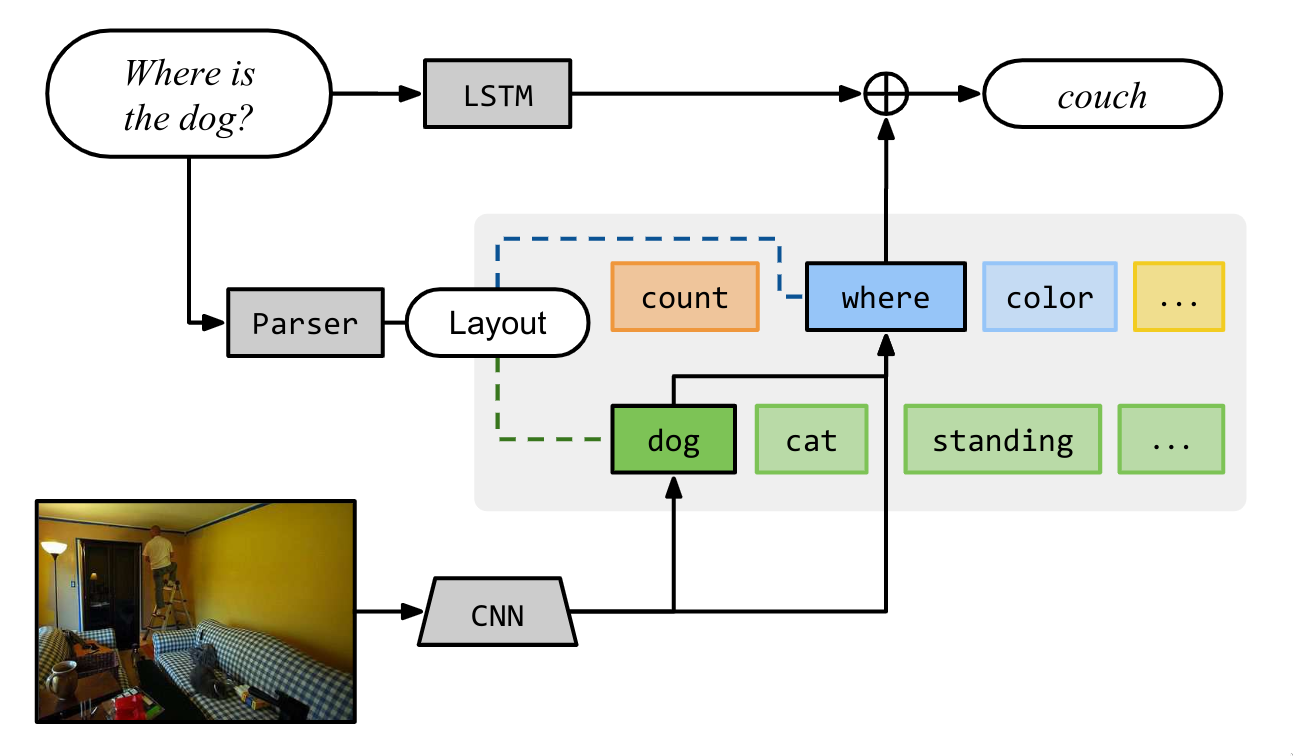
\includegraphics[width=0.75\textwidth]{module_network.png}
    \caption[A Neural Module Network VQA Model \cite{andreas2016neural}]{\citeauthor{andreas2016neural} propose the Neural Module Network \cite{andreas2016neural}, in which reasoning operations are strung together based on parser outputs and use combinations and transformations of attention maps on image features to predict a final answer to the question.}
    \label{fig:andreas2016neural_neural_module_network}
\end{figure}

\citeauthor{andreas2016learning} \cite{andreas2016learning} improve upon their earlier work with a more robust method for generating compositional module layouts from questions, combining LSTM embeddings of the question with representations of candidate module layouts to select a module layout using a reinforcement learning approach. This model sees only a slight improvement over their previous iteration, however provides a novel framework for a variety of graph-based reasoning tasks; the scene graphs and functional programs in CLEVR and GQA are strong supervisory training data for such models, and recent scene graph generation techniques would prove useful in generalising models to images that have not been previously annotated.

\section{Model Performance Summary}

\subsection{VQAv2.0}

\begin{table}[htbp]
    \centering
    \begin{tabularx}{\linewidth}{@{\extracolsep{4pt}} l C C C C C C C C @{}}
        \hline
        \multirow{2}{*}{\textbf{Model}} & \multicolumn{4}{c}{Test-dev} & \multicolumn{4}{c}{Test-std} \\
        \cline{2-5}\cline{6-9}
        & All & Yes/No & Num. & Other & All & Yes/No & Num. & Other \\
        \hline
        % Fusion
        BLOCK \cite{ben2019block} & 67.58 & 83.6 & 47.33 & 58.51 & 67.92 & 83.98 & 46.77 & 58.79 \\
        \hline
        % Attention
        % Graph
    \end{tabularx}
    \caption{A comparison of various models for different question types on the VQA v2.0 dataset.}
\end{table}

\subsection{CLEVR}

% \begin{table}[htbp]
%     \centering
%     \begin{tabularx}{\linewidth}{@{\extracolsep{4pt}} l C C C C C @{}}
%         \hline
%         \multirow{2}{*}{\textbf{Model}} & \multicolumn{4}{c}{Test-dev} & Test-std \\
%         \cline{2-5}\cline{6-6}
%         & Y/N & Number & Other & All & All \\
%         \hline
%         MAC \cite{hudson2018compositional} & & & & & \\
%         \hline
%     \end{tabularx}
%     \caption{A comparison of various models on the VQA dataset the accuracy metric.}
% \end{table}

\subsection{GQA}

\begin{table}[htbp]
    \centering
    \begin{tabularx}{\linewidth}{@{\extracolsep{4pt}} l C C C @{}}
        \hline
        \multirow{2}{*}{\textbf{Model}} & \multicolumn{3}{c}{Test} \\
        \cline{2-4}
        & Binary & Open & All \\
        \hline
        % Fusion
        BLOCK \cite{ben2019block} & - & - & - \\
        \hline
    \end{tabularx}
    \caption{A comparison of various models for different question types on the GQA test set using the accuracy metric.}
\end{table}

\begin{table}[htbp]
    \begin{tabularx}{\linewidth}{@{\extracolsep{4pt}} l C C C C C C @{}}
        \hline
        \multirow{2}{*}{\textbf{Model}} & \multicolumn{6}{c}{Test} \\
        \cline{2-7}
        & Distribution & Grounding & Validity & Plausibility & Consistency & Accuracy \\
        \hline
        % Fusion
        BLOCK \cite{ben2019block} & - & - & - & - & - & - \\
        \hline
    \end{tabularx}
    \caption{A comparison of various models on the GQA test set for multiple metrics.}
\end{table}

